\documentclass[11pt,wide]{article}

\usepackage{polski}
\usepackage[utf8]{inputenc}

\usepackage{graphicx} % Required to insert images
\usepackage{listings} % Required for insertion of code

\usepackage{mathtools}
\usepackage{amsthm}


\title{Analiza numeryczna (M) - Pracownia 0 \\ Zadanie P0.11\\
Tekst, wzory i wartości}
\date{Wrocław, Listopad 12, 2019}
\author{Jakub Kuciński}

\begin{document}

\maketitle
\thispagestyle{empty} 
\tableofcontents

\section{Wprowadzenie}
Wzór Taylora -- przedstawienie funkcji (n+1)-razy różniczkowalnej za pomocą wielomianu zależnego od kolejnych jej pochodnych oraz dostatecznie małej reszty. Twierdzenia mówiące o możliwości takiego przedstawiania pewnych funkcji (nawet dość abstrakcyjnych przestrzeni) noszą zbiorczą nazwę twierdzeń Taylora od nazwiska angielskiego matematyka Brooka Taylora, który opublikował pracę na temat lokalnego przybliżania funkcji rzeczywistych w podany niżej sposób. Ta własność funkcji różniczkowalnych znana była już przed Taylorem -- w 1671 odkrył ją James Gregory. 

\section{Twierdzenie Taylora}
Niech Y będzie przestrzenią unormowaną oraz  \({\displaystyle f: [a,b]\to Y}\)  będzie funkcją (n+1)-razy różniczkowalną na przedziale [a,b] w sposób ciągły (na końcach przedziału zakłada się różniczkowalność z lewej, bądź odpowiednio, z prawej strony). Wówczas dla każdego punktu x z przedziału (a,b) spełniony jest wzór zwany wzorem Taylora:

\newtheorem*{mydef}{Twierdzenie}

\begin{mydef} Wzór Taylora.\\
\(f(x) = \displaystyle\sum_{k=0}^{n} \left( \frac{(x-a)^k}{k!} f^{(k)}(a) \right) + R_n (x, a)\) 
gdzie \(R_n\) spełnia zależność:\\
\(\displaystyle\lim\limits_{x \to a} \frac{R_n(x,a)}{(x-a)^n} = 0\)

\end{mydef}



\section{Reszty we wzorze Taylora wyrażone w sposób jawny}
\subsection{Reszta w postaci całkowej}
\(\displaystyle R_n(x,a)=\int_a^x \mathrm{\frac{{(x-t)}^{n}}{n!}} f^{(n+1)}(t)\mathrm{d}t  \)
\subsection{Reszta w postaci Lagrange'a}
Istnieje takie \(\theta\in [0,1]\), że\\
\(\displaystyle R_n(x,a)=\frac{(x-a)^{n+1}}{(n+1)!}f^{(n+1)}(a+\theta(x-a))   \)
\subsection{Reszta w postaci Cauchy'ego}
Istnieje takie \(\theta\in [0,1]\), że\\
\(\displaystyle R_n(x,a)=\frac{(x-a)^{n+1}}{n!} (1-\theta)^n f^{(n+1)}(a+\theta(x-a))   \)

\section{Mniej lub bardziej przypadkowe liczby w tabeli}
\begin{center}
  \begin{tabular}{ | l | c  r | }
    \hline
      & 2321 & 3 \\ \hline
    42 & 553 & 676 \\ 
    742608 & 834 & 96 \\
    \hline
  \end{tabular}
\end{center}

\section{Wykres}
\begin{figure}[h]
	\centering
	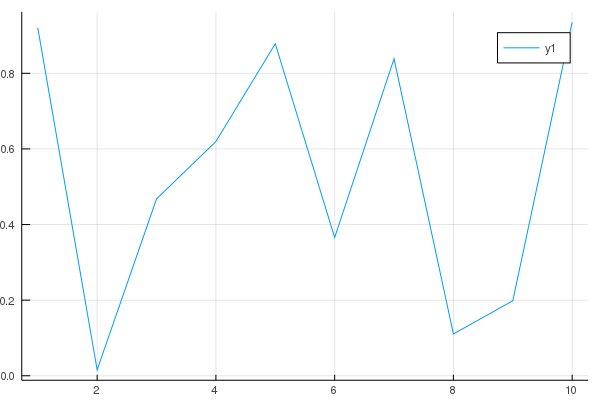
\includegraphics[width=0.82\textwidth]{plot}
	\caption{Wykres funkcji \(f(x)\)}
\end{figure}


\end{document}